\section{Anadefi}
\subsection{Présentation d'Anadefi}
Anadefi est le progiciel leader en France pour l’analyse financière de comptes d’entreprises s’appuyant sur près de quinze ans d’existence et d’expérience. Conçu spécifiquement pour les banques et établissements financiers, il s’inscrit comme un outil essentiel du suivi et de la maîtrise du risque de contrepartie.\\

{Anadefi est un progiciel complet intégrant :}
\begin{itemize}
\item analyse de bilans
\item analyse de comptes de résultat
\item ratios
\item notation
\item score
\item prévisionnel, simulations
\item comparaison d’entreprises
\item analyse des risques liés (dirigeant commun à plusieurs sociétés …)
\item gestion des groupes d’entreprises
\item comparaisons sectorielles
\item rapport d’analyse permettant d’intégrer dans un même document, des informations quantitatives (extraites automatiquement d’Anadefi), et des éléments qualitatifs (saisis par les analystes).
\item Module d’instruction de crédit avec notation à l’opération
\item Module d’historisation conforme aux accords de Bâle II
\item Module de centrale de bilans.\\
\end{itemize}

Anadefi se plie aux exigences de leurs clients.
{Les clients Anadefi ont la possibilité de paramétrer :}
\begin{itemize}
\item les informations en saisie (liasses fiscales, documents comptables …)
\item l’ensemble des calculs financiers
\item la forme et le contenu des documents à éditer (dossier de présentation pour décision, surveillance …)\\
\end{itemize}

{\large{Une réponse aux réseaux bancaires décentralisés:}}\\
Pour répondre à la problématique des réseaux bancaires décentralisés, Anadefi permet de définir un cadre commun d’analyse à tout le groupe, tout en permettant des adaptations locales (par région ou pays).\\

{\large{Gestion des prospects (dossiers éphémères):}}\\
Parce que l’analyse du risque de contrepartie concerne aussi les prospects, Anadefi intègre des "dossiers éphémères", avec la possibilité de les intégrer dans le système d’information lorsqu’ils deviennent clients.

\newpage
{\large{Anadefi Un module optionnel assure la conformité}} 
 avec les exigences du ratio McDonough (ratio prudentiel des banques) – Bâle 2
\begin{itemize}
\item Historisation événementielle
\item Reconstitution d’environnements
\item Back-testing
\item Matrices de transition
\item Pistes d’audit
\item Alimentation des applicatifs externes\\
\end{itemize}
{\large{Anadefi un progiciel tous secteurs:}}

\begin{itemize}
\item Grandes entreprises (groupes internationaux)
\item PME-PMI
\item Professions libérales
\item Commerçants
\item Artisans
\item Agriculture
\item Immobilier
\item Collectivités locales et territoriales
\item Associations
\item Établissements financiers\\
\end{itemize}

{\large{Anadefi un progiciel pour l’international:}}
\begin{itemize}
\item Multi-devises (indépendance entre la devise de 
saisie et la devise d’affichage, double affichage, conversion automatique)
\item Multilingue
\item Comptes tous pays\\
\end{itemize}

{\large{Anadefi Un progiciel ouvert:\\}}
Anadefi dispose d’une interface intégrée avec les principales banques de données comptables et financières sur les entreprises (Coface-SCRL, Dun \& Bradstreet, BIL, Bilans Services, Sysiphe …).\\

{\large{En option :\\}}
module EDI pour intégration directe des comptes sociaux.\\

{\large{Gestion des habilitations en fonction des profils utilisateurs:\\}}
Selon les utilisateurs, vous pouvez restreindre l’utilisation d’Anadefi à certaines fonctions : pour un déploiement sans risque dans tout votre réseau.\\

{\large{Atouts techniques:}}
\begin{itemize}
\item Serveur d’application full IP pour des liaisons fiables et éprouvées, aux standards du marché.
\item Postes clients sans procédure d’installation, ce qui facilite le déploiement des nouvelles versions d’Anadefi et réduit les coûts.
\item Optimisation des flux sur la bande passante.\\
\end{itemize}

\newpage

{\large{Clients Anadefi :}}\\
Crédit Mutuel de Bretagne, Crédit Agricole SA (accords nationaux) / Caisses d’Epargne (accords nationaux) / CCF (accords nationaux) / Groupe Crédit Mutuel Bretagne / A3C / Alsabaïl / Bank of Hawaï / Bankoa / Banque Calédonienne d’Investissement / Banque de la Réunion / Banque de Nouvelle Calédonie / Banque de Picardie / Banque des Savoie / Banque Hervet / Bankoa / CCSO / Chaix / CA CIB / Dupuy de Parseval / Expanso / Financière Oceor / Groupama Assurance Crédit / Marze /Pelletier / SMC / Socredo /Eurofactor / Unigrain / Banque Centrale des Etats d’Afrique Centrale


\subsection{Architecture}

L'architecture est composée d'un serveur Ades, c'est à ce serveur que les clients vont se connecter pour effectuer leurs opérations.\\

D'un serveur d'archivage, qui va permettre d'archiver leurs données en cas de perte ou d'une éventuelle extraction.\\

Et il y a un service qui va faire le lien entre ces deux serveurs qui est le producteur notamment pour recalculer et indexer la base de données.\\

\begin{figure}[h]
\centering
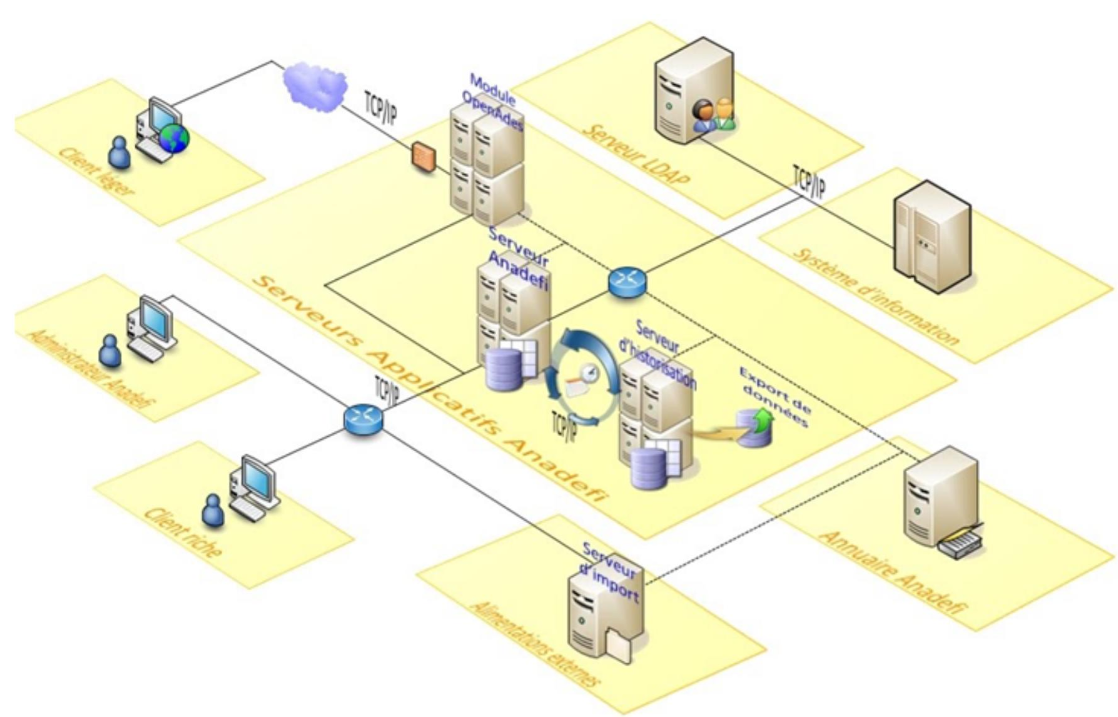
\includegraphics[scale=0.6]{resources/architecture.png}
\caption{Architecture Anadefi}
\label{ArchiAnadefi}
\end{figure}

\subsection{Gestionnaire d'instance}

Le gestionnaire d'instance est un outil qui va nous permettre d'avoir plusieurs instances du progiciel Anadefi avec chacun son propre serveur Ades, producteur et archivage.\\

L'avantage c'est qu'on peut avoir le paramétrage de chaque client et de switcher facilement d'une instance à une autre en un rien de temps.\\

Concrètement, tous les clients Anadefi n'ont pas les mêmes critères d'évaluations et de scoring en terme d'analyse financière et d'évaluation du risque. Pour pouvoir les administrer il aurait donc fallu installer le paramétrage d'un client d'abord, paramétrer, une fois terminé, désinstaller puis recommencer pour faire la même chose pour le deuxième, troisième client etc, on s'y perd très rapidement. C'est donc la raison pour laquelle on utilise le gestionnaire d'instance car il va nous permettre d'avoir plusieurs instances pour les différents clients Anadefi.

\subsection{Les outils Anadefi}

Il y a plus d'une vingtaine d'outils qui permettent de paramétrer le progiciel Anadefi.
Chaque serveur a ses propres outils pour paramétrer et configurer ces derniers.\\

Pour créer ou modifier un paramétrage on passe par un outil qui sert à administrer la base de données Anadefi qui est "Admin2000.exe". Il est destiné à un administrateur fonctionnel en charge de renseigner les nomenclatures des différentes listes déroulantes de l’application cliente, le paramétrage des grilles d'analyse, des grilles de saisie, les documents de sortie EDW\footnote{c'est un document similaire à Word}, les systèmes de cotations et de scoring.\\

Une fois que le paramétrage est crée ou modifié, on lance un autre outil "packager.exe" qui va créer un fichier avec l'extension .ppa qui contiendra toutes les nomenclatures, grilles d'analyse, de saisie, EDW etc, qu'on a paramétré au préalable sur admin2000.exe.\\

Pour que ce paramétrage soit effectif, on va utiliser un autre outil appelé "deployer.exe" qui va appliquer ce .ppa à l'instance correspondante, toutes les configurations faites par l'administrateur fonctionnel.\\

Une fois le paramétrage déployé, on va utiliser un dernier outil qui va mettre en production ce paramétrage, c'est l'outil "devprod.exe". Une fois utilisé, le paramétrage fait par l'administrateur est en place.\\

Il y a encore plusieurs outils qui permettent de paramétrer ou d'administrer le progiciel Anadefi.


